% Modelo de Dissertação do Mestrado em Informática da PUC - Alterado para cumprir a normalização de 2011
\documentclass[a4paper,brazil,ruledheader,normaltoc,capchap,twoside,openany]{abnt_pucmg_utf8}

\let\cleardoublepage\clearpage

\usepackage{titlesec}
\titleformat{\chapter}[hang]{\huge\bfseries}{\thechapter}{1em}{}
\titlespacing*{\chapter}{0pt}{*0}{20pt} % Ajusta espaçamentos antes/depois do capítulo

% Pacotes e configurações adicionais
\usepackage[a4paper,left=3cm,right=2cm,top=3cm,bottom=2cm]{geometry}
\usepackage[printonlyused]{acronym}
\usepackage{multirow}
%\usepackage[alf, abnt-emphasize=em, abnt-thesis-year=title]{abntcite}
\usepackage{abnt-PPGInf-PUCMG}
\usepackage{graphicx}
\usepackage{float}
\usepackage[symbol]{footmisc}
\usepackage[all]{xy}
\usepackage{url,amsmath}
\usepackage{amssymb}
\usepackage[portuguese, linesnumbered, ruled, vlined]{algorithm2e}
\usepackage{algorithmic}
\usepackage{listings}
\usepackage{setspace}
\usepackage{rotating}
\usepackage{array}
\usepackage{longtable}
\usepackage{colortbl}
\usepackage[size=normalsize,labelfont=bf,textfont={bf},labelsep=endash]{caption}
\captionsetup[subfloat]{labelfont=bf,textfont={bf}}
\usepackage{paralist}
\captionsetup{figurewithin=none}
\captionsetup{tablewithin=none}
\setlength{\LTcapwidth}{\textwidth}
\setcounter{tocdepth}{3}
\setcounter{secnumdepth}{3}
\usepackage{subfig}

\usepackage[backend=biber,style=abnt]{biblatex}
\addbibresource{referencias.bib} % Replace 'referencias.bib' with your .bib file name


% Configuração de código-fonte
\lstset{extendedchars=\true,
 inputencoding=utf8,
 literate={\$}{{\$}}1,
 commentstyle=\it,
 stringstyle=\bf,
 belowcaptionskip=5pt,
 numbers=left,
 stepnumber=1,
 firstnumber=1,
 numberstyle=\tiny,
 breaklines=true,
 frame=tb,
 basicstyle=\footnotesize,
 stringstyle=\ttfamily,
 showstringspaces=false,
 mathescape,
 tabsize=3
}


\renewcommand{\lstlistingname}{Código}
\renewcommand{\lstlistlistingname}{Lista de Códigos}
%\citeoption{abnt-etal-cite=1, abnt-and-type=e}

% Ajuste de espaçamento para títulos e listas
\makeatletter
\renewcommand\numberline[1]{
	\leftskip 0em
	\rightskip 1.6em
	\parfillskip -\rightskip
	\parindent 0em
	\@tempdima 2.0em
	\vspace{0em} \advance\leftskip \@tempdima \null\nobreak\hskip -\leftskip
	%FIGURA
    \normalfont #1 -- }
\makeatother

\begin{document}

% Para forçar que elementos pré-textuais sejam impressos no anverso da folha
\setboolean{@twoside}{false}

\autor{Felipe Vilhena Dias \\ Gabriel Cunha Schlegel}

% Título do trabalho
\titulo{Técnicas de Renderização em Tempo Real para Jogos Digitais: Avanços e Desafios}

% Comentário
\comentario{Projeto de Pesquisa apresentado na disciplina Trabalho Interdisciplinar III - Pesquisa Aplicada do curso de Ciência da Computação da Pontifícia Universidade Católica de Minas Gerais.}

% Instituição
\instituicao{Ciência da Computação \par Instituto de Ciências Exatas e Informática \par Pontifícia Universidade Católica de Minas Gerais}

% Local e Data
\local{Belo Horizonte}
\data{2024}

% Capa e Folha de Rosto
\capa
\setboolean{@twoside}{true}
\folhaderosto

% Resumo Extenso
\begin{resumo}
A renderização em tempo real é essencial no desenvolvimento de jogos digitais modernos, permitindo gráficos de alta qualidade que respondem às interações do usuário. Entre as principais técnicas destacam-se rasterização avançada, \textit{ray tracing}, oclusão de ambiente e algoritmos de sombreamento. O \textit{ray tracing} em tempo real trouxe avanços significativos em realismo, porém enfrenta desafios de desempenho. Soluções híbridas que combinam \textit{ray tracing} com rasterização têm sido empregadas para equilibrar qualidade visual e taxa de quadros.

Outro aspecto importante é a \textit{Global Illumination} (GI), que utiliza abordagens como \textit{Reflective Shadow Maps} (RSM), \textit{Screen Space Reflections} (SSR) e \textit{Screen Space Ambient Occlusion} (SSAO) para simular iluminação indireta e reflexos. O avanço das GPUs modernas, com núcleos dedicados ao \textit{ray tracing}, tem possibilitado a execução eficiente dessas técnicas.

Desafios persistem na otimização do desempenho, sendo aplicadas técnicas como \textit{Level of Detail} (LoD) e \textit{culling} para manter uma boa taxa de quadros. Tendências futuras incluem o uso de inteligência artificial e \textit{cloud gaming} para aprimorar a renderização. Conclui-se que o equilíbrio entre qualidade gráfica e desempenho será alcançado por meio de inovações em algoritmos e hardware.


\vspace{0.5cm}
\noindent \textbf{Palavras-chave:} Renderização em Tempo Real, Jogos Digitais, Ray Tracing, GPUs, Técnicas de Sombreamento, Otimização.
\end{resumo}

% Sumário
\tableofcontents

% Altera para espaçamento 1,5 a partir daqui
\onehalfspacing

% TEXTUAIS
\setboolean{@twoside}{true}
\setcounter{page}{7}

% Capítulo de Introdução
\chapter{Introdução}

A renderização em tempo real é uma técnica que permite a geração de imagens com alta qualidade e velocidade, essencial para criar experiências imersivas em jogos digitais. Com o avanço das tecnologias de hardware e software, desenvolvedores de jogos têm sido capazes de alcançar níveis de realismo visual que eram inimagináveis há apenas alguns anos. Essas técnicas não apenas melhoram a aparência dos jogos, mas também influenciam diretamente a jogabilidade e a experiência do usuário, criando mundos virtuais que são visualmente impressionantes e responsivos às ações dos jogadores.

*“O campo da renderização em tempo real tem visto avanços significativos, especialmente com a introdução do ray tracing em tempo real, que promete transformar a maneira como os gráficos são processados em jogos”* (Smith, 2020). Esta citação destaca a importância das novas técnicas de renderização que estão sendo exploradas atualmente, como o ray tracing em tempo real, que permite simular de forma precisa a interação da luz com os objetos em uma cena, criando efeitos de iluminação e sombras extremamente realistas. No entanto, a implementação dessas técnicas traz consigo desafios significativos, como a necessidade de otimização para manter o desempenho necessário para uma experiência de jogo fluida.

% Capítulos subsequentes
\setboolean{@openright}{false}
\makeatletter
\renewcommand{\chapter}{%
  \if@openright\cleardoublepage\else\clearpage\fi % Remove quebra padrão
  \secdef{\@chapter}{\@schapter}}
\makeatother


\titleformat{\chapter}[hang]{\huge\bfseries}{\thechapter}{1em}{}
\titlespacing*{\chapter}{0pt}{*0}{20pt} % Ajusta espaçamentos antes/depois do capítulo

\chapter{Revisão Bibliográfica}

A renderização em tempo real tem evoluído significativamente no desenvolvimento de jogos digitais, abrangendo algoritmos de rasterização, técnicas de sombreamento e, mais recentemente, a introdução do \textit{ray tracing} em tempo real. Esta seção analisa os principais conceitos e avanços que moldaram o estado da arte na renderização em tempo real, destacando seu impacto no desempenho e na qualidade visual dos jogos.

\begin{figure}[h!]
    \centering
    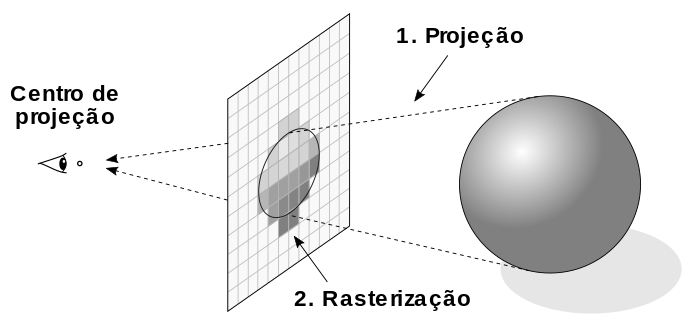
\includegraphics[width=0.7\textwidth]{04_rasterization.png}
    \label{fig:Rasterizaçao - Diagrama}
    
    \cite{RDiagram}
\end{figure}
\section{Rasterização}

A rasterização é a técnica predominante para a renderização em tempo real em jogos, devido à sua eficiência computacional. Este processo envolve a conversão de cenas tridimensionais em imagens bidimensionais, calculando a cor de cada pixel com base nos objetos visíveis na tela.\cite{RTR} a rasterização é especialmente adequada para aplicações que requerem altas taxas de quadros, como jogos, pois pode ser otimizada para ser executada diretamente no hardware das GPUs modernas.

Entretanto, a rasterização tem limitações na simulação de efeitos de iluminação complexos, como reflexos e refrações. Para contornar essas limitações, desenvolvedores utilizam técnicas complementares, como \textit{Screen Space Ambient Occlusion} (SSAO) e \textit{Screen Space Reflections} (SSR), que ajudam a simular oclusão de ambiente e reflexos de maneira mais convincente \cite{MCGuire:2011}.





\section{Ray Tracing em Tempo Real}

\begin{figure}
    \centering
    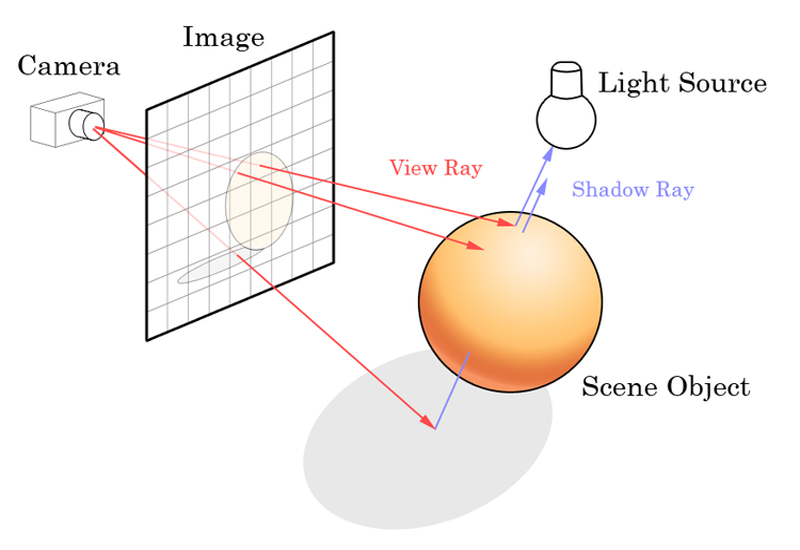
\includegraphics[width=0.5\linewidth]{Cara-Kerja-Ray-Tracing.jpg}
    \label{fig:RTX - Diagrama}
    
    \cite{RTDiagram}
\end{figure}

O \textit{ray tracing} em tempo real emergiu como uma das inovações mais significativas nos gráficos digitais. Diferente da rasterização, o \textit{ray tracing} simula com maior precisão a interação da luz com os objetos em uma cena, proporcionando reflexos, sombras e refrações mais realistas. Historicamente, o \textit{ray tracing} convencional era inviável para jogos devido ao seu alto custo computacional, sendo amplamente utilizado em filmes e animações pré-renderizadas \cite{PBR}



Com o advento de GPUs equipadas com núcleos dedicados ao \textit{ray tracing}, como as da arquitetura Turing da NVIDIA, essa técnica se tornou viável em tempo real, embora ainda com limitações de desempenho. Assim, em Hybrid Rendering for Real-Time Ray Tracing \cite{Barré-Brisebois2019}, uma solução híbrida que combina o ray tracing para efeitos específicos (como reflexos em superfícies metálicas) e a rasterização para o restante da cena tem se mostrado eficaz para equilibrar qualidade visual e desempenho. 
\\
\\
\\
\\
\\
\\\\\\\\

\section{Global Illumination}

\begin{figure}
    \centering
    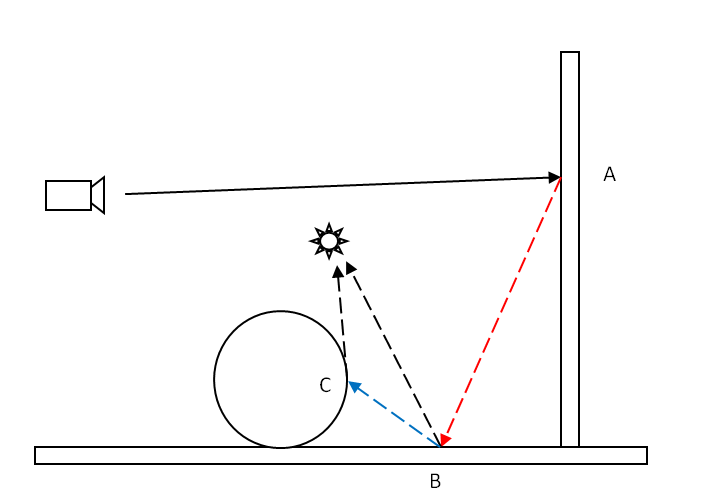
\includegraphics[width=0.45\linewidth]{GI.png}
    \label{fig:RTX - Diagrama}

    \cite{GIDiagram}
\end{figure}

Um conceito essencial na renderização em tempo real é o de \textit{Global Illumination} (GI), que trata da interação indireta da luz em uma cena, simulando múltiplas reflexões e criando ambientes mais realistas. \cite{Dachsbacher2005} discutem a técnica conhecida como \textit{Reflective Shadow Maps} (RSM), que aproxima a iluminação indireta com base em mapas de sombras refletidas.

Entretanto, as técnicas de GI podem ser computacionalmente exigentes, representando um desafio significativo para a renderização em tempo real. Abordagens como \textit{pre-computed radiance transfer} (PRT) e mapas de iluminação são utilizadas para aliviar parte desse custo, permitindo que a iluminação de cenas estáticas seja precalculada, como discutido por \cite{IR:1997}.

\section{Otimização de Desempenho}

Um dos principais desafios na renderização em tempo real é otimizar o desempenho sem comprometer a qualidade visual. Para garantir uma experiência de jogo fluida, técnicas como \textit{Level of Detail} (LoD) e \textit{frustum culling} são amplamente utilizadas. O LoD ajusta a complexidade dos objetos de acordo com sua proximidade à câmera, enquanto o \textit{frustum culling} elimina objetos não visíveis na cena, reduzindo a carga de processamento \cite{LoD}.

As arquiteturas de GPUs multicore desempenham um papel crucial ao permitir o paralelismo em larga escala, fundamental para atender às crescentes demandas gráficas dos jogos \cite{SIEGEL19873}. Além disso, a integração de técnicas de \textit{machine learning} e a exploração de renderização baseada em nuvem (\textit{cloud gaming}) emergem como tópicos promissores, com o potencial de melhorar ainda mais o desempenho gráfico em jogos futuros \cite{Keller2018}.

\section{Conclusão}

A revisão bibliográfica revela que a renderização em tempo real é um campo dinâmico, impulsionado por avanços em hardware e algoritmos. O \textit{ray tracing} em tempo real destaca-se como uma técnica inovadora, embora enfrente desafios de desempenho que precisam ser superados. Técnicas de otimização como LoD, SSAO, SSR, juntamente com GPUs de última geração, são essenciais para equilibrar qualidade visual e taxa de quadros, um fator crítico para a experiência de jogo. O futuro dessa área promete soluções ainda mais sofisticadas, incluindo a aplicação de inteligência artificial na renderização e o desenvolvimento de tecnologias de renderização baseadas em nuvem.
\makeatletter
\renewcommand{\chapter}{%
  \if@openright\cleardoublepage\else\clearpage\fi % Remove quebra padrão
  \secdef{\@chapter}{\@schapter}}
\makeatother
\chapter{Metodologia}
\label{metodo}

Este capítulo descreve as etapas metodológicas adotadas na condução do projeto de pesquisa. As atividades foram planejadas para garantir uma abordagem sistemática e consistente. A Figura \ref{fig-metodologia} ilustra o fluxo metodológico adotado.

\begin{figure}[h]
\centering
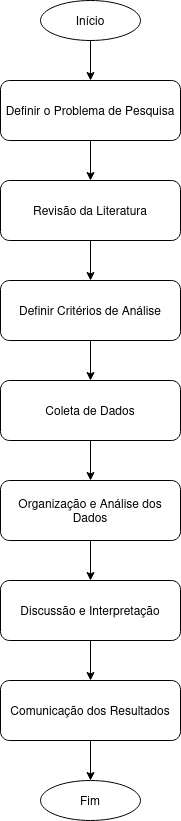
\includegraphics[width=0.3\textwidth]{imagem/metodologia.drawio.png}
\caption{Fluxo metodológico da pesquisa.}
\label{fig-metodologia}
\end{figure}


\section{Atividades a serem realizadas}
Nesta seção, detalhamos as atividades planejadas para o desenvolvimento do projeto.

\subsection{Atividade 1: Definir o problema de pesquisa}
A primeira atividade consiste na definição do problema de pesquisa, delimitando o tema e os objetivos específicos, com base em uma questão central que guiará o estudo.

\subsection{Atividade 2: Revisão da literatura}
A segunda atividade envolve uma revisão bibliográfica abrangente, buscando fundamentar teoricamente o problema e identificar lacunas na literatura.

\subsection{Atividade 3: Definir critérios de análise}
Nessa etapa, são estabelecidos os critérios que orientarão a coleta e análise dos dados, de forma a garantir consistência e validade no tratamento das informações.

\subsection{Atividade 4: Coleta de dados}
A coleta de dados será realizada utilizando técnicas específicas, como entrevistas, questionários ou análise documental, conforme o objetivo da pesquisa.

\subsection{Atividade 5: Organização e análise dos dados}
Os dados coletados serão organizados e analisados seguindo os critérios previamente definidos, utilizando métodos qualitativos e/ou quantitativos.

\subsection{Atividade 6: Discussão e interpretação}
Nessa etapa, os resultados obtidos serão discutidos e interpretados, relacionando-os aos objetivos iniciais e à literatura revisada.

\subsection{Atividade 7: Comunicação dos resultados}
Finalmente, os resultados serão comunicados por meio da elaboração de relatórios, artigos científicos e/ou apresentações.

\section{Cronograma}
A Tabela \ref{tab-crono} apresenta o cronograma das atividades descritas anteriormente, organizadas ao longo dos meses de execução do projeto.

\begin{table}[h]
\centering
\caption{Cronograma}
\label{tab-crono}
\begin{tabular}{|l|l|l|l|l|}
\hline
\textbf{Atividade} &
\textbf{\begin{tabular}[c]{@{}l@{}}Meses\\ 1-3\end{tabular}} &
\textbf{\begin{tabular}[c]{@{}l@{}}Meses\\ 4-6\end{tabular}} &
\textbf{\begin{tabular}[c]{@{}l@{}}Meses\\ 7-9\end{tabular}} &
\textbf{\begin{tabular}[c]{@{}l@{}}Meses\\ 10-11\end{tabular}} \\ \hline
Definição do problema & X &   &   &   \\ \hline
Revisão da literatura & X & X &   &   \\ \hline
Definir critérios      &   & X &   &   \\ \hline
Coleta de dados        &   &   & X &   \\ \hline
Análise dos dados      &   &   & X & X \\ \hline
Discussão              &   &   &   & X \\ \hline
Comunicação            &   &   &   & X \\ \hline
\end{tabular}
\end{table}

\makeatletter
\renewcommand{\chapter}{%
  \if@openright\cleardoublepage\else\clearpage\fi % Remove quebra padrão
  \secdef{\@chapter}{\@schapter}}
\makeatother
\chapter{Avanços na Renderização em Tempo Real}

Os avanços tecnológicos na renderização em tempo real têm transformado o desenvolvimento de jogos digitais, permitindo experiências visuais imersivas e de alta qualidade. Este capítulo explora os principais avanços recentes, incluindo o desenvolvimento de hardware especializado, técnicas híbridas e o uso de inteligência artificial para otimizações.

\section{Tecnologias Emergentes no Hardware}
A introdução de GPUs com núcleos dedicados para \textit{Ray Tracing} em tempo real, como as séries RTX da NVIDIA, marcou um ponto de virada na computação gráfica. Essas tecnologias possibilitam a geração de iluminação, sombras e reflexos realistas sem o impacto de desempenho presente nas abordagens anteriores.

Além disso, arquiteturas mais eficientes, como a série RDNA da AMD, oferecem suporte avançado para técnicas de renderização híbrida, combinando rasterização com traçado de raios, otimizando o desempenho para plataformas de diferentes capacidades.

\section{Integração de Machine Learning}
O uso de inteligência artificial tem desempenhado um papel crucial na renderização moderna. Algoritmos de \textit{Deep Learning} são empregados em técnicas como o \textit{Deep Learning Super Sampling} (DLSS), que melhora a qualidade da imagem renderizada enquanto reduz a carga computacional.

Por meio do aprendizado de padrões visuais, a IA é capaz de prever e gerar detalhes em tempo real, otimizando o uso de recursos e garantindo uma experiência visual mais fluida.

\section{Renderização Baseada em Nuvem}
A renderização em nuvem é uma solução que permite ultrapassar as limitações de hardware local. Com o processamento gráfico sendo realizado em servidores remotos, os jogadores podem acessar gráficos de alta qualidade em dispositivos menos potentes. Serviços como GeForce NOW e Google Stadia demonstram o potencial dessa abordagem para democratizar o acesso a experiências visuais avançadas.

No entanto, essa tecnologia ainda enfrenta desafios relacionados à latência e à dependência de conexões estáveis e de alta velocidade.

\section{Otimizações em Engines de Jogos}
As engines modernas, como Unreal Engine 5 e Unity, têm incorporado avanços tecnológicos para facilitar a implementação de renderização em tempo real. Ferramentas como o \textit{Nanite}, presente na Unreal Engine 5, permitem renderizar geometrias extremamente detalhadas sem comprometer o desempenho, enquanto o \textit{Lumen} oferece iluminação global dinâmica de alta qualidade.

Essas inovações estão tornando a criação de ambientes visuais complexos mais acessível para desenvolvedores, reduzindo a barreira de entrada para estúdios independentes.

\section{Contribuições para a Experiência do Jogador}
Os avanços discutidos neste capítulo têm impacto direto na experiência dos jogadores. A melhoria na fidelidade visual e a redução de artefatos gráficos contribuem para maior imersão e realismo, enquanto otimizações em tempo real garantem que o desempenho seja consistente, mesmo em cenários complexos.

Essas inovações não apenas elevam o nível dos jogos atuais, mas também abrem possibilidades para o futuro da indústria de jogos digitais, integrando gráficos realistas a experiências interativas e narrativas mais envolventes.


\makeatletter
\renewcommand{\chapter}{%
  \if@openright\cleardoublepage\else\clearpage\fi % Remove quebra padrão
  \secdef{\@chapter}{\@schapter}}
\makeatother
\chapter{Desafios da Renderização em Jogos Digitais}

Apesar dos avanços tecnológicos, a renderização em tempo real ainda enfrenta desafios significativos. Este capítulo aborda as principais limitações, desde questões técnicas até impactos ambientais, destacando a busca constante por soluções equilibradas que mantenham a qualidade visual sem comprometer o desempenho.

\section{Limitações Computacionais}
As técnicas modernas, como \textit{Ray Tracing} em tempo real e \textit{Global Illumination}, exigem alto poder de processamento. Mesmo com a evolução das GPUs, o custo computacional dessas abordagens pode ser proibitivo, especialmente em plataformas de menor capacidade, como consoles de gerações anteriores ou dispositivos móveis.

O desafio está em otimizar os algoritmos para aproveitar ao máximo os recursos disponíveis, reduzindo a carga computacional sem perder qualidade.

\section{Qualidade Visual vs. Desempenho}
Uma das maiores dificuldades na renderização em jogos é equilibrar a qualidade visual com o desempenho. Enquanto os jogadores esperam gráficos realistas e imersivos, a taxa de quadros por segundo (FPS) é crucial para garantir uma experiência fluida.

Muitas vezes, os desenvolvedores precisam realizar concessões, priorizando desempenho em detrimento de efeitos visuais avançados, especialmente em títulos multijogador onde a fluidez é essencial.

\section{Escalabilidade em Jogos Multijogador}
Jogos multijogador massivos enfrentam desafios únicos na renderização. A necessidade de sincronizar milhares de objetos e jogadores em tempo real impõe uma carga adicional sobre o sistema, dificultando a manutenção de gráficos de alta qualidade.

Além disso, a escalabilidade entre diferentes plataformas, de PCs de ponta a consoles menos potentes, adiciona uma camada extra de complexidade para os desenvolvedores.

\section{Sustentabilidade Energética}
Com a crescente demanda por gráficos mais realistas, o consumo energético das GPUs também aumenta. Isso levanta preocupações ambientais, especialmente em contextos de data centers que suportam renderização em nuvem.

A busca por soluções sustentáveis, como arquiteturas de hardware mais eficientes e algoritmos que economizem energia, tornou-se uma prioridade para muitos estúdios e fabricantes de hardware.

\section{Desafios de Implementação}
Embora as ferramentas modernas, como engines de jogos, ofereçam suporte avançado para renderização, implementar técnicas sofisticadas ainda requer conhecimento técnico especializado. Isso pode limitar a adoção dessas tecnologias por estúdios menores ou desenvolvedores independentes.

\section{Reflexão Sobre os Desafios}
Os desafios descritos neste capítulo destacam a complexidade inerente à renderização em tempo real. A indústria de jogos está em constante evolução, e superar essas barreiras exige inovação contínua, colaboração entre fabricantes de hardware e desenvolvedores de software, e uma abordagem equilibrada entre tecnologia, arte e sustentabilidade.


\makeatletter
\renewcommand{\chapter}{%
  \if@openright\cleardoublepage\else\clearpage\fi % Remove quebra padrão
  \secdef{\@chapter}{\@schapter}}
\makeatother
\chapter{Estudos de Caso e Aplicações Práticas}

Neste capítulo, serão explorados exemplos práticos e estudos de caso que demonstram a aplicação de técnicas avançadas de renderização em jogos digitais. Essas análises destacam como tecnologias inovadoras foram utilizadas para criar experiências visuais marcantes, além de discutir os desafios enfrentados durante sua implementação.

\section{Jogos com Ray Tracing}
O \textit{Ray Tracing} em tempo real tem se tornado um diferencial visual em jogos modernos. Títulos como \textit{Cyberpunk 2077}, \textit{Control} e \textit{Minecraft RTX} exemplificam como essa tecnologia pode transformar a iluminação, os reflexos e as sombras, elevando a qualidade visual.

Esses jogos enfrentaram desafios relacionados ao desempenho, especialmente em hardware menos potente, mas ilustram o potencial do \textit{Ray Tracing} quando combinado com técnicas como \textit{Deep Learning Super Sampling} (DLSS).

\section{Implementação Híbrida}
A combinação de técnicas tradicionais, como rasterização, com métodos modernos, como \textit{Ray Tracing}, é uma abordagem comum para equilibrar qualidade e desempenho. Em jogos como \textit{Fortnite} e \textit{Call of Duty: Modern Warfare}, técnicas híbridas foram utilizadas para maximizar a qualidade visual enquanto mantinham altas taxas de quadros por segundo.

Essa abordagem permite que desenvolvedores adaptem a experiência para diferentes plataformas, desde PCs de alto desempenho até consoles menos poderosos.

\section{Global Illumination em Jogos}
A iluminação global (\textit{Global Illumination}) é um componente chave para criar ambientes realistas. Jogos como \textit{The Last of Us Part II} e \textit{Horizon Forbidden West} empregaram essa técnica para simular interações complexas de luz, criando cenários imersivos e ricos em detalhes.

Embora a iluminação global tradicional seja computacionalmente intensiva, tecnologias como \textit{Lumen}, na Unreal Engine 5, estão tornando-a mais acessível em tempo real.

\section{Integração com Realidade Virtual e Aumentada}
A renderização em tempo real também é essencial para experiências de realidade virtual (VR) e aumentada (AR). Títulos como \textit{Half-Life: Alyx} demonstram como a fidelidade gráfica, combinada com baixa latência, é crucial para manter a imersão em VR.

Além disso, jogos de AR, como \textit{Pokémon GO}, mostram como a renderização otimizada pode ser usada para integrar elementos virtuais ao mundo real.

\section{Reflexões sobre os Estudos de Caso}
Os jogos analisados demonstram o impacto direto das técnicas de renderização no sucesso comercial e na recepção crítica. Embora os avanços tecnológicos tenham permitido criar experiências mais imersivas, eles também ressaltam a importância de equilibrar inovação com viabilidade técnica e desempenho.


\makeatletter
\renewcommand{\chapter}{%
  \if@openright\cleardoublepage\else\clearpage\fi % Remove quebra padrão
  \secdef{\@chapter}{\@schapter}}
\makeatother
\chapter{Discussão dos Resultados}

Neste capítulo, será realizada uma análise detalhada dos resultados obtidos ao longo do estudo das técnicas de renderização em tempo real aplicadas aos jogos digitais. A discussão aborda as principais descobertas, comparando-as com a literatura existente, e considera as implicações práticas para desenvolvedores e jogadores.

\section{Análise das Técnicas de Renderização}
Ao longo do estudo, observou-se que as técnicas de renderização em tempo real, como o \textit{Ray Tracing} e a \textit{Global Illumination}, têm contribuído significativamente para a qualidade visual dos jogos, proporcionando um nível de realismo sem precedentes. No entanto, esses avanços também apresentam desafios, como o alto custo computacional e a necessidade de otimizações constantes para manter o desempenho em níveis aceitáveis.

Comparando com os estudos revisados, os resultados obtidos indicam que, embora os desenvolvedores tenham feito progressos na implementação dessas técnicas, a adaptação às diferentes plataformas continua a ser uma barreira importante. Jogos como \textit{Cyberpunk 2077}, que utilizam \textit{Ray Tracing} em tempo real, exemplificam essa dualidade, pois, embora proporcionem gráficos de alta qualidade, exigem hardware de ponta para garantir um desempenho fluido.

\section{Desempenho x Qualidade Visual}
A relação entre desempenho e qualidade visual continua sendo um dos principais dilemas enfrentados pelos desenvolvedores. A pesquisa revelou que, para muitos jogos modernos, a implementação de técnicas avançadas de renderização compromete o desempenho em plataformas com hardware limitado. No entanto, o uso de tecnologias como o \textit{DLSS} e as implementações híbridas de \textit{Ray Tracing} têm demonstrado que é possível alcançar um equilíbrio entre esses dois aspectos, embora com a necessidade de realizar ajustes finos em cada plataforma.

Por exemplo, em jogos como \textit{Call of Duty: Modern Warfare}, a utilização de técnicas híbridas conseguiu melhorar a qualidade visual sem impactar significativamente o desempenho, uma abordagem que pode ser vista como uma solução viável para jogos de alta intensidade gráfica.

\section{Sustentabilidade e Eficiência Energética}
Outro ponto de destaque nesta pesquisa foi a questão da sustentabilidade. Com a crescente demanda por gráficos de alta qualidade, o consumo energético das GPUs tem aumentado, o que levanta preocupações ambientais. O estudo mostrou que as soluções de renderização em nuvem e a evolução das arquiteturas de hardware mais eficientes são essenciais para reduzir o impacto ambiental.

Embora as soluções baseadas em nuvem, como o Google Stadia, ainda enfrentem desafios relacionados à latência e à conectividade, elas representam um passo importante em direção à otimização energética no desenvolvimento de jogos, permitindo que dispositivos menos potentes acessem gráficos avançados sem sobrecarregar os sistemas locais.

\section{O Futuro da Renderização em Jogos Digitais}
A análise dos resultados também aponta para um futuro promissor para a renderização em tempo real, impulsionado pela adoção de inteligência artificial, como o uso de IA para melhorar a qualidade da imagem em tempo real (por meio de técnicas como o \textit{DLSS}) e pela evolução contínua das GPUs. Espera-se que, no futuro, a implementação de \textit{Ray Tracing} se torne mais acessível, permitindo que uma maior gama de dispositivos suporte esses gráficos avançados.

Além disso, a integração de novas tecnologias, como o uso de redes neurais para otimização de renderização e a melhoria na integração com plataformas de Realidade Virtual e Aumentada, pode criar novas formas de interação e imersão para os jogadores.

\section{Implicações Práticas para os Desenvolvedores}
Por fim, os resultados desta pesquisa têm implicações práticas importantes para os desenvolvedores de jogos. A necessidade de otimização constante, a escolha de técnicas híbridas e a consideração das especificações de hardware das plataformas alvo são fatores cruciais para garantir uma experiência de jogo satisfatória.

Desenvolvedores devem considerar o uso de técnicas como \textit{Ray Tracing} de forma equilibrada, optando por implementações híbridas que permitam um bom desempenho, sem abrir mão da qualidade visual, especialmente em jogos multijogador onde a fluidez é essencial.


\makeatletter
\renewcommand{\chapter}{%
  \if@openright\cleardoublepage\else\clearpage\fi % Remove quebra padrão
  \secdef{\@chapter}{\@schapter}}
\makeatother
\chapter{Conclusão e Trabalhos Futuros}

Neste capítulo, são apresentadas as conclusões do estudo sobre técnicas de renderização em tempo real para jogos digitais, bem como as sugestões para trabalhos futuros que podem expandir ou aprofundar as questões discutidas. A análise foi baseada nos avanços recentes, desafios persistentes e nas aplicações práticas dessas técnicas no desenvolvimento de jogos.

\section{Conclusões}
A renderização em tempo real tem se consolidado como um dos pilares da experiência imersiva em jogos digitais. Técnicas avançadas como \textit{Ray Tracing}, \textit{Global Illumination}, e o uso de inteligência artificial, como o \textit{Deep Learning Super Sampling} (DLSS), possibilitaram avanços significativos na qualidade visual dos jogos, resultando em gráficos mais realistas e dinâmicos. No entanto, essas inovações também introduzem desafios técnicos, principalmente em relação ao alto custo computacional e à necessidade de equilibrar desempenho e qualidade visual, especialmente em plataformas mais limitadas.

Além disso, os desafios relacionados ao consumo de energia das GPUs e a sustentabilidade na renderização em tempo real também são questões que precisam ser abordadas para garantir que os avanços não comprometam o meio ambiente ou a acessibilidade dos jogos a um público maior.

A implementação de técnicas híbridas, que combinam métodos tradicionais com técnicas modernas, tem mostrado ser uma abordagem promissora para alcançar o equilíbrio entre qualidade e desempenho. A crescente adoção dessas técnicas pelos desenvolvedores de jogos, juntamente com o desenvolvimento de hardwares mais eficientes, indica um futuro promissor para a renderização em tempo real.

\section{Trabalhos Futuros}
Embora este estudo tenha fornecido uma visão abrangente sobre as técnicas de renderização em tempo real e seus desafios, ainda existem várias áreas que merecem aprofundamento em pesquisas futuras. Alguns dos possíveis caminhos incluem:

\begin{itemize}
    \item \textbf{Otimização de Algoritmos de Ray Tracing:} A busca por algoritmos mais eficientes que reduzam o custo computacional do \textit{Ray Tracing} e que possam ser aplicados em uma maior variedade de dispositivos, incluindo consoles e dispositivos móveis, é uma área crítica de pesquisa.
    
    \item \textbf{Renderização Adaptativa:} Investigar novas abordagens para renderização adaptativa, que ajustem a qualidade visual dinamicamente com base nos recursos disponíveis do sistema, garantindo uma experiência consistente em diversas plataformas.
    
    \item \textbf{Integração de IA na Renderização:} Explorar o uso de redes neurais e outras técnicas de inteligência artificial para otimizar a renderização em tempo real, como a utilização de IA para predição de iluminação ou para melhorar a qualidade de texturas e sombras.
    
    \item \textbf{Impacto Ambiental da Renderização:} Estudar soluções mais sustentáveis para reduzir o impacto ambiental da renderização em tempo real, explorando o uso de tecnologias como a renderização em nuvem ou otimizações de hardware que reduzam o consumo energético.
    
    \item \textbf{Experiências Imersivas em Realidade Virtual e Aumentada:} A pesquisa de técnicas de renderização otimizadas para ambientes de realidade virtual (VR) e aumentada (AR) pode criar novas fronteiras de interação no universo dos jogos, proporcionando experiências ainda mais imersivas.
    
    \item \textbf{Aplicações em Jogos Multijogador:} A renderização em tempo real em jogos multijogador massivos continua sendo um desafio devido à sincronização de gráficos em tempo real para múltiplos jogadores. Pesquisas focadas em melhorar o desempenho gráfico sem comprometer a sincronização e a fluidez serão essenciais para o desenvolvimento de novos jogos multijogador.
\end{itemize}

Essas áreas de pesquisa podem não apenas aprimorar as técnicas de renderização, mas também expandir as possibilidades de criação de mundos virtuais mais imersivos e acessíveis.

\section{Considerações Finais}
A renderização em tempo real continua a ser um campo dinâmico e de grande importância no desenvolvimento de jogos digitais. Com o rápido avanço das tecnologias, como o \textit{Ray Tracing} e a renderização baseada em inteligência artificial, o futuro da indústria de jogos parece promissor. No entanto, é fundamental que os desenvolvedores considerem tanto os desafios técnicos quanto as questões ambientais e de acessibilidade para garantir uma evolução sustentável e inclusiva.

A busca por soluções que permitam a renderização de gráficos impressionantes em dispositivos de diferentes capacidades, sem sacrificar o desempenho ou a sustentabilidade, será crucial para o futuro dos jogos digitais. Assim, a colaboração contínua entre as comunidades de pesquisa e indústria, juntamente com a inovação tecnológica, será a chave para superar os desafios atuais e explorar novas possibilidades no campo da renderização em tempo real.
14414

% Bibliografia
\renewcommand{\bibname}{Referências}
\printbibliography


% Apêndices e Anexos (se necessário)
%\setboolean{@openright}{true}
%\apendice
%\begin{apendice}
%\include{pos-texto/apendiceA}
%\end{apendice}

%\anexo
%\include{pos-texto/anexo}

\end{document}
